Esse capítulo tem como objetivo mostrar a metodologia utilizada para atingir o objetivo do trabalho. A Figura \ref{figure:metodologia} mostra, de maneira geral, o esquema da metodologia proposta. Primeiramente, será discutido o ambiente de experimento. Em seguida, será explicitado como os dados foram pré-processados. Por último, será discutido a escolha e implementação dos modelos e as métricas de avaliação utilizadas, assim como qual foi o ambiente de teste utilizado.

\begin{figure}
    \centering
    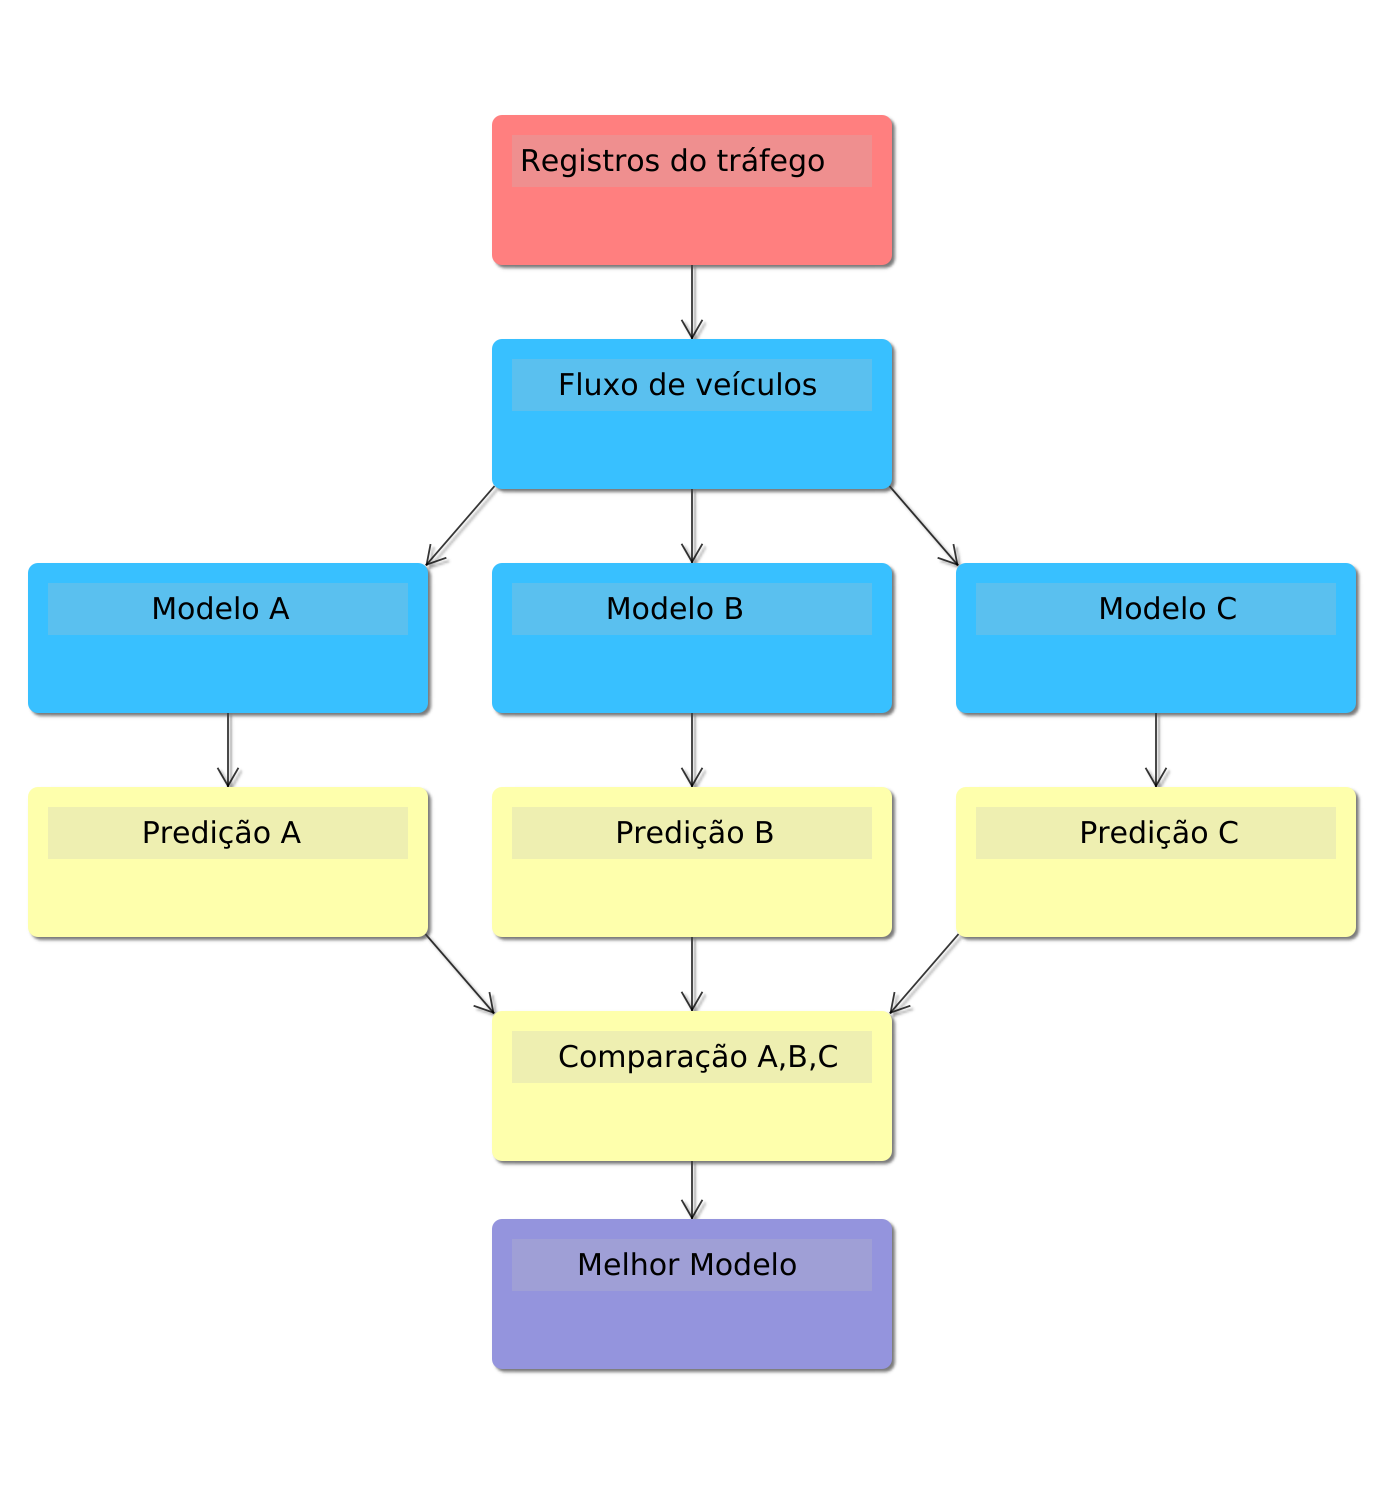
\includegraphics[scale=0.4]{monography/img/tccFlux.png}
    \label{figure:metodologia}
    \caption[Fluxograma da metodologia]{Fluxograma da metodologia}
\end{figure}

\section{Ambiente de Experimento}

O ambiente de experimento foi um servidor equipado com Ubuntu 64 bits. O servidor possui dois CPUs \textit{Intel(R) Xeon(R) Platinum 8160 CPU @ 2.10GHz} e 251 GiB de memória principal. Cada CPU dessas possui 24 núcleos e executa até 48 \textit{threads} em paralelo. No total então são 96 \textit{threads}, que foram usados paralelamente para acelerar a execução do experimento. Porém, em algumas partes da execução, menos \textit{threads} tiveram que ser usadas, pois não havia memória principal o suficiente para todas as instâncias em paralelo.

\section{Pré-Processamento dos Dados}

Nesta etapa serão feitos ajustes no conjunto de dados inicial, como remoções de inconsistências e transformações nos dados mostrados na Tabela \ref{table:data}. Esse ajustes têm como propósito melhorar a aprendizagem dos modelos que serão utilizados. Subsequentemente, será mostrado como os conjuntos de treino e teste foram criados a partir do conjunto de dados e das variações do modelo. Por fim, é realizado uma exploração da sazonalidade do fluxo.

\subsection{Limpeza dos Dados}

No conjunto de dados inicial existem colunas que não são relevantes para o problema, ou possuem algum tipo de inconsistência. Devido a este fato, as colunas a seguir serão removidas:

\begin{itemize}
    \item \texttt{Faixa}
    \item  \texttt{Hora}
    \item \texttt{Limite de Velocidade da Via}
    \item  \texttt{Tamanho do Veículo}
\end{itemize}

A coluna \texttt{Faixa} será removida, pois nas transformações que virão a seguir, esse dado se tornará desnecessário, visto que o objetivo deste trabalho é prever o fluxo na via como um todo e não em faixas específicas. A coluna \texttt{Hora} será removida, pois com o intervalo de fluxo, já é possível saber a qual momento do dia se refere determinado registro. Além disso, para utilizar a hora propriamente dita como entrada dos modelos, seria necessária uma análise mais minuciosa de como tratá-la, o que foge do escopo definido pelo trabalho. A coluna \texttt{Limite de Velocidade da Via} será removida, pois este dado tem seu valor repetido ao longo de todos os registros, isto é, o valor é constante em todo o conjunto de dados e não afeta no treinamento dos modelos. A coluna \texttt{Tamanho do Veículo} será removida, pois não foi medida de forma precisa, visto que existem registros com veículos de tamanho zero (o que não é fisicamente possível).

\subsection{Transformação dos Dados}

A transformação dos dados se torna útil quando um tipo de dado pode ser representado de outra forma, em geral mais simples, que ajude no treinamento do modelo. No caso, a coluna \texttt{Data} será transformada, pois existem diversas informações subtendidas em uma data como dia da semana, se é feriado, início ou fim do mês, entre outros. Essas informações que podem ser extraídas de uma data podem ter uma relação direta ou indireta com o comportamento de uma via. Visto que a quantidade de dados que temos não chega nem a cobrir todas as datas de 1 ano, se torna difícil para os modelos aprenderem a extrair e utilizar essas informações. 

Sendo assim, a coluna \texttt{Data} será simplificada para o dia da semana, dado que o fluxo aparenta apresentar comportamentos similares nos mesmos dias da semana. Para evitar falsas suposições do modelo, será utilizado a técnica \textit{one hot encoding} para transformar essa coluna \texttt{Data} e 7 colunas diferentes (uma para cada dia da semana). Cada uma dessas colunas terá valores 1 ou 0 para representar se é ou não um certo dia da semana. Isso é necessário, pois caso fosse uma coluna quantitativa (0 representando domingo e 1 representando segunda, por exemplo) o modelo poderia realizar inferências, como "segunda" é maior que "quarta", ou analogias similares.

\subsection{Acumulação dos registros}

Como visto na literatura, existem algumas maneiras de se fazer a predição de veículos em uma via. Seja pelo fluxo, pela densidade, ou pela velocidade média dos carros, por exemplo. Neste trabalho, optou-se por utilizar o fluxo como método de predição, seguindo o padrão visto em \cite{lana_2018}.

Sendo assim, o conjunto de dados será transformado de uma série temporal de registros de veículos para uma série temporal de fluxos. Isto é, será calculado a quantidade de veículos que passaram por um local em um determinado intervalo de tempo. Além disso, também foram calculadas a velocidade média e a densidade no mesmo intervalo. Para definir o intervalo que foi utilizado, testou-se os valores de intervalo para 2.5, 5 e 7.5 minutos. Note que foram utilizados intervalos que sejam múltiplos de 15, visto que todos os tempos de predição no futuro serão múltiplos de 15.

É preciso levar em consideração que quando se acumula os registros em um intervalo de tempo muito pequeno, o conjunto de dados apresenta muito ruído, dificultando a aprendizagem e afetando a qualidade da previsão. Em contrapartida, ao se aumentar o intervalo, o conjunto de dados pode se tornar muito pequeno, o que também pode dificultar a aprendizagem.

Para se escolher qual dos intervalos seria o melhor para a predição, o tamanho do intervalo de fluxo será um dos parâmetros a serem escolhidos. Isto é, será realizado uma comparação entre os modelos para ver como que eles reagem. Abaixo também pode ser observado parte do código responsável por realizar esta transformação:

\begin{algorithm}[H]
\Entrada{o proprio texto}
\Saida{como escrever algoritmos com \LaTeX2e }
\Inicio{
inicializa\c{c}\~ao\;
\Repita{fim do texto}{
leia o atual\;
\uIf{entendeu}{
vá para o próximo\;
próximo se torna o atual\;}
\Else{volte ao início da seção\;}
}
}
\caption{Como escrever algoritmos no \LaTeX2e}
\end{algorithm}

\begin{lstlisting}[language=Python, caption = GetFlow Python Function]
def get_flow (data, flow_interval, normalize, verbosity):
  date = np.asarray(data['Date'])
  weekDay = np.asarray(data['WeekDay'])
  time = np.asarray(data['Time'])
  speed = np.asarray(data['Speed'])
  
  dateControl = date[0]
  timeBlock = flow_interval
  countFlow = 0
  accSpeed = 0
  flowData = []

  for i in range(len(date)):
    if time[i] >= timeBlock: # init a new time block
      flowData.append(get_flow_data(countFlow, accSpeed, weekDay[i])) 
      timeBlock += flow_interval
      accSpeed = 0
      countFlow = 0
      
    if date[i] > dateControl: # reset on day change
      dateControl = date[i]
      timeBlock = flow_interval 
      countFlow = 0
      accSpeed = 0
      
    if time[i] < timeBlock: # add car on flow
      countFlow += 1
      accSpeed += speed[i]

  return flowData

\end{lstlisting}

\begin{table}[H]
    \begin{tabular}{cccccccccc}
    \toprule
    \multicolumn{1}{l}{\textbf{Flow}} & \multicolumn{1}{l}{\textbf{Density}} & \multicolumn{1}{l}{\textbf{Average Speed}} & \multicolumn{1}{l}{\textbf{Sun}} &
    \multicolumn{1}{l}{\textbf{Mon}} & \multicolumn{1}{l}{\textbf{Tue}} & \multicolumn{1}{l}{\textbf{Wed}} & \multicolumn{1}{l}{\textbf{Thu}} &
    \multicolumn{1}{l}{\textbf{Fri}} &
    \multicolumn{1}{l}{\textbf{Sat}} \\
    \midrule
     6 & 0.260870 & 23.500000 & 0 & 0 & 0 & 0 & 0 & 0 & 1 \\
    \midrule
    17 & 0.586207 & 29.235294 & 0 & 0 & 0 & 0 & 0 & 0 & 1 \\
    \midrule
    15 & 0.625000 & 24.933333 & 0 & 0 & 0 & 0 & 0 & 0 & 1 \\
    \midrule
    18 & 0.666667 & 27.500000 & 0 & 0 & 0 & 0 & 0 & 0 & 1 \\
    \midrule
    14 & 0.736842 & 19.500000 & 0 & 0 & 0 & 0 & 0 & 0 & 1 \\
    \midrule
    14 & 0.700000 & 20.571429 & 0 & 0 & 0 & 0 & 0 & 0 & 1 \\
    \midrule
     6 & 0.352941 & 17.833333 & 0 & 0 & 0 & 0 & 0 & 0 & 1 \\
    \midrule
     8 & 0.400000 & 20.375000 & 0 & 0 & 0 & 0 & 0 & 0 & 1 \\
    \midrule
    11 & 0.550000 & 20.181818 & 0 & 0 & 0 & 0 & 0 & 0 & 1 \\
    \midrule
    15 & 0.652174 & 23.466667 & 0 & 0 & 0 & 0 & 0 & 0 & 1 \\
    \midrule
    10 & 0.588235 & 17.700000 & 0 & 0 & 0 & 0 & 0 & 0 & 1 \\
    \midrule
    13 & 0.722222 & 18.769231 & 0 & 0 & 0 & 0 & 0 & 0 & 1 \\
    \midrule
    11 & 0.785714 & 14.363636 & 0 & 0 & 0 & 0 & 0 & 0 & 1 \\
    \midrule
     8 & 0.400000 & 20.125000 & 0 & 0 & 0 & 0 & 0 & 0 & 1 \\
    \midrule
     8 & 0.347826 & 23.750000 & 0 & 0 & 0 & 0 & 0 & 0 & 1 \\
    \bottomrule
    \end{tabular}
    \label{table:data_pre}
    \caption{Amostra do pré-processamento dos dados ao se utilizar 7.5 minutos de intervalo do sensor RSI128}
\end{table}

No final do pré-processamento o resultado possuirá 3 colunas quantitativas e 7 qualitativas. As colunas de \textit{Density} e \textit{Average Speed} são contínuas e a coluna \textit{Flow} é discreta. As outras 7 colunas representam uma classificação indicando se é ou não (0 representa falso e 1 verdadeiro) um certo dia da semana, sendo assim uma coluna qualitativa ordinal.

Vale notar que, como o período é o mesmo para qualquer um dos sensores, ao se acumular os registros, o tamanho do conjunto de dados será sempre igual. Isto é, será equivalente ao intervalo de tempo do conjunto de dados, 92 dias, divido pelo tempo de agregação de fluxo (7.5 minutos), o que gera 17.664 registros de fluxo dos 536.879 registros de passagem de veículos disponíveis.

\subsection{Normalização dos Dados}
% TODO: adicionar referência do porque normalizar dados
Na área de aprendizagem de máquina, é comum vermos modelos de predições para diferentes tipo de variáveis. Por vezes, os valores assumidos por essas variáveis podem apresentar um domínio grande demais, como no caso da predição de valores de ações da bolsa de valores. Com valores em um intervalo tão grande, o treinamento dos modelos tende a piorar. Para contornar este problema, é comum utilizar técnicas que visam diminuir o intervalo de valores que as variáveis podem assumir. Uma destas técnicas é a normalização. 

Em um dos tipos da normalização, utiliza-se o maior e o menor valor que o seu conjunto de dados atinge para ajustar os valores intermediários. Por exemplo, o maior fluxo calculado foi 94 veículos para o sensor \textbf{RSI128} com acumulação de 7,5 minutos e o menor foi 0. Assim, foram ajustados os valores do conjunto de dados dentro de um intervalo entre 0 e 1, com 0 representando o menor valor e 60, o maior valor. Porém, os testes realizados mostraram que a normalização não trouxe melhorias significativas para as predições deste trabalho, apresentando, inclusive, resultados levemente piores em alguns modelos. Por este motivo, optou-se por continuar os experimentos sem normalização.

\subsection{Criação dos Conjunto de Treino e Teste}

Será utilizado o conjunto dos dados pré-processados (\(D\)) para gerar o conjunto de dados de treino (\(X\)) e teste (\(Y\)). Cada elemento (\(x_i\)) do conjunto de treino  será uma série temporal dos atributos. Essa série temporal representa uma visão contínua limitada do passado ao presente momento. Ou seja, cada elemento de treino será uma subsequência de \(D\) de tamanho \(m\), com cada instância (\(x_{i, j}\)) será uma das linhas da Tabela \ref{table:data_pre}. Para o conjunto de testes, cada elemento (\(y_i\)) será o fluxo no futuro (\(x_{i + k, m_{flow}}\)). Para fins de análise, será utilizado o conjunto de treino para gerar um outro mais simples. Este possuirá somente o fluxo, permitindo assim verificar se as colunas de \texttt{Average Speed}, \texttt{Density} e as de dias da semana melhoram a performance do modelo. 

Os modelos no entanto não possuem uma entrada parecida. Logo, é necessário adaptar o conjunto de testes os modelos. Uma versão será para os modelos de aprendizagem profunda (\textit{\acrshort{LSTM}} e \textit{\acrshort{GRU}}) com três dimensões (amostras por passos por atributos), assim como mostrado acima. A outra versão será para os modelos tradicionais (\textit{\acrshort{RF}} e \textit{\acrshort{SVM}}), que terá somente duas dimensões (amostras por atributos). Ou seja, \(x'_i\), nesse caso, não é uma lista de tupla e sim somente uma tupla com todos os elementos da lista de tupla.

\subsection{Sazonalidade dos dados}

Na Figura \ref{figure:flow_discution} é mostrado o resultado da agregação dos registros de veículos em um intervalo de 7.5 minutos. É possível observar que existem flutuações na quantidade de fluxo de veículo de acordo com o dia. Este fato fica mais evidente se observarmos o primeiro pico do gráfico, referente ao Domingo, pois este apresenta um menor fluxo de veículos, o que é esperado que aconteça em um dia não comercial. Isso mostra que os dados apresentam certa sazonalidade. Esta sazonalidade se manifesta em várias escalas, no gráfico mostrado é possível ver apenas a sazonalidade referente aos dias da semana, mas ela também se aplica, por exemplo, a semana do mês, ao mês do ano, etc. Por este motivo, o escopo deste trabalho foi definido apenas para os 3 meses de dados disponíveis. 


\begin{figure}
    \centering
    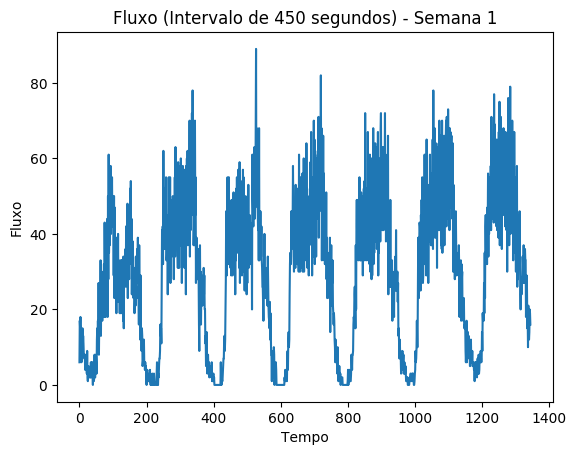
\includegraphics[scale=1]{monography/img/flows/flow_450_week_01.png}
    \label{figure:flow_discution}
    \caption[Fluxo da Primeira Semana]{Fluxo da Primeira Semana}
\end{figure}

\section{Modelos Desenvolvidos}

Visto que a predição do fluxo é o foco do trabalho, que temos um conjunto de pares entrada e saída, e que que o fluxo é quantitativo. Será utilizado técnicas de aprendizagem de máquina supervisionadas de regressão para prever a curto prazo o fluxo da via. Dentre essas técnicas, podemos dividi-las novamente em paramétricos e não-paramétricos.

Dos modelos não-paramétricos, se destacam o \textit{\acrfull{LSTM}} e o \textit{\acrfull{GRU}}, sendo ambos \textit{\acrshort{RNN}}'s. Quanto ao \textit{\acrfull{LSTM}}, vale ressaltar que existem diversas variações e implementações. Porém, segundo Greff et. al. \cite{Greff_2015} as variações da \textit{\acrshort{LSTM}} não possuem tantas diferenças quanto a qualidade de suas previsões. Por este motivo, este trabalho utilizou o \textit{\acrfull{LSTM}} comum. Dos modelos paramétricos, o mais utilizado na literatura para previsão de fluxo é o \textit{\acrfull{ARIMA}} e suas variações \cite{doi:10.1080/01441647.2014.992496}, além de modelos mais simples como \textit{\acrfull{LR}}. 

% TODO: falar que estamos utilizando um modelo para cada tipo de viés (rf para arvores, etc)

Todos os modelos não-paramétricos citados foram implementados para este trabalho. Quanto aos modelos paramétricos, foram testados dois modelos, sendo eles o \textit{\acrshort{ARIMA}} e o \textit{\acrshort{LR}}. Porém, ambos tiveram resultados inferiores em relação aos modelos não-paramétricos testados, sendo que ambos estavam utilizando os parâmetros padrões da biblioteca \textit{StatModels}. Além disso, \textit{\acrshort{ARIMA}} se mostrou extremamente custosos computacionalmente de se treinar e otimizar. Por estes dois motivos citados, os modelos paramétricos foram retirados dos experimentos.

\subsection{Modelos de Comparação}

Serão utilizados também dois modelos com o único propósito de estabelecer uma base de comparação inicial para os outros modelos. Serão eles o \textit{Naive} e \textit{Moving Average}. O primeiro faz suas predições apenas escolhendo o valor de fluxo mais recente dos que recebeu de entrada. Já o segundo faz a média dos valores de fluxo recebidos na entrada. Dessa forma, é possível colocar em perspectiva o desempenho dos modelos escolhidos. Também fora implementado o \textit{Random Guess} cujo respondia aleatoriamente para qualquer entrada (valores entre o menor e maior elemento encontrado no conjunto), porém este era muito inferior e decidimos retirá-lo.

\subsection{Implementação}

As arquiteturas utilizadas neste trabalho foram implementados na linguagem \textit{Python} utilizando bibliotecas como \textit{Keras} com \textit{TensorFlow} e \textit{SKLearn}. Decidiu-se por utilizar essas bibliotecas, pois suas implementações já são robustas, otimizadas e bem testadas. Implementar todos os modelos sem o auxílio de nenhuma biblioteca seria ineficiente para objetivo dos experimentos e prono a erros. Além disso, o uso das bibliotecas facilita a reprodução dos experimentos para os interessados em avançar ou verificar este projeto.

\textit{Keras} foi utilizado para implementar os modelos de \textit{\acrshort{LSTM}} e \textit{\acrshort{GRU}} e optou-se por usar como base dessa biblioteca o \textit{TensorFlow}, visto que este é o \textit{framework} com suporte para aprendizado de máquina mais utilizado dentre os desenvolvedores, segundo um questionário feito em 2018 pelo \textit{Stack Overflow} \cite{stack_2018}. Já \textit{SKLearn} foi utilizado para implementar os modelos \acrshort{RF} e \acrshort{SVM}. Além disso, utilizou-se a biblioteca \textit {SKLearn} para realizar uma pesquisa dos melhores parâmetros e hiper-parâmetros.

\subsection{Escolha de Parâmetros e Hiper-Parâmetros}

Tanto os modelos quando o conjunto de treinamento podem ser ajustados para servir mais ao problema. Sendo assim, esse trabalho realiza testes para tentar melhorar a predição dos modelos. Primeiramente será feito a escolha dos parâmetros para determinar, dentre as opções escolhidas, quais os melhores parâmetros de ajuste do conjunto de treinamento. Subsequentemente será feita a escolha dos hiper-parâmetros que varia de modelo para modelo. Vale notar que as opções a serem testadas precisam lidar com limitações de hardware.

A escolha de parâmetros será feita assumindo que os parâmetros são independentes. Elas são o passado visível, o número de divisões do conjunto de dados e o tamanho do intervalo do fluxo. O passado visível determina o tamanho do entrada, o número de divisões afeta o tamanho das amostras de treino e teste e o tamanho do intervalo do fluxo altera o tamanho do conjunto de dados de uma forma geral. Na literatura a escolha de parâmetros é empírica e baseada no problema, sendo assim baseamos no nosso problema para determinar os valores a serem testados, sendo eles:

\begin{itemize}
    \item \textbf{Número de divisões do conjunto de dados} \textit{Blocking}: 1, 2, 4, 8 divisões;
    \item \textbf{Passado Visível}: 60, 120, 240 e 480 minutos;
    \item \textbf{Tamanho do Intervalo Acumulado}: 150, 300, 450 segundos;
\end{itemize}

Para o número de divisões e passado visível é utilizado uma escala exponencial para ter uma noção de como essas variáveis afetam a medida que vão crescendo. Número de divisões tem seu máximo como 8, pois divisões muito maiores fariam com que o conjunto de treinamento tivesse menos de 1 semana. Passado visível tem seu máximo como 480 minutos por limitações de hardware. Já tamanho do intervalo acumulado é limitado a divisores de 15 minutos, visto que o trabalho tem como objetivo prever como o fluxo vai estar após 15, 30, 45 e 60 minutos. Além disso, tempos de acumulação inferiores tornam o dado muito ruidoso e tempo de acumulação superior torna o conjunto de dados muito pequeno.

A escolha de hiper-parâmetros será utilizada para verificar a sensibilidade dos modelos com os hiper-parâmetros antes escolhidos. Para essa fase, o conjunto de testes é divido em dois novamente (treino e teste \textit{tuning}). Isso é feito para evitar sobre-ajuste e os resultados finais sejam genéricos o suficiente para casos nunca visto antes. Para estes será feita uma busca total entre os parâmetros escolhidos, isto é, todos com todos. 

Para os modelos de aprendizagem profunda (\textit{\acrshort{LSTM}} e \textit{\acrshort{GRU}}) os hiper-parâmetros são os mesmos. Segundo Greff et. al. \cite{Greff_2015}, que realizou extensos testes nesses dois modelos, chegou a conclusão que os dois fatores que mais afetam o aprendizado dos modelos são a taxa de aprendizado e o tamanho da rede. Sendo assim, esses dois foram escolhidos como os hiper-parâmetros, com as opções sendo:

\begin{itemize}
    \item \textbf{Taxa de Aprendizado}: 0.001, 0.004, 0.016 e 0.064;
    \item \textbf{Número de Células da Rede}: 50, 75, 100, 125 células;
\end{itemize}

A taxa de aprendizado tem uma escala exponencial sendo que o menor valor se baseia no valor padrão escolhido pelo biblioteca \textit{Keras}. Já o número de células da rede é limitada pelo hardware, visto que se tem um crescimento computacional significativo ao se aumentar o número de células. 

Para \textit{\acrshort{RF}} os hiper-parâmetros foram escolhidos para evitar o sobre-ajuste seguindo, em parte, a sugestão de Trevor Hastie et al. \cite{hastie2005elements} para construção de árvores e variando a quantidade de estimadores. Sendo assim, os hiper-parâmetros escolhidos foram a quantidade de estimadores (árvores) e altura máxima das árvores. A quantidade de estimadores e a altura máxima das árvores foram escolhido também um escala exponencial para ver como o modelo reage a medida que os valores crescem.  Sendo os valores escolhidos:

\begin{itemize}
    \item \textbf{Quantidade de Estimadores}: 50, 100, 200, 400, 800 estimadores;
    \item \textbf{Altura Máxima}: 8, 16, 32, 64 e sem limitações no tamanho;
\end{itemize}

% TODO: terminar SVM
Para \textit{\acrshort{SVM}} os hiper-parâmetros ...

\begin{itemize}
    \item \textbf{C}: 1, 10, 100 e 1000;
    \item \textbf{\(\gamma\)}: 4 valores espaçados, do espaço logarítmico de -2 a 2, e o padrão da biblioteca; 
\end{itemize}

\section{Avaliação Final}

Na literatura é comum serem utilizados as métricas \textit{\acrfull{RMSE}} e \textit{\acrfull{MAPE}}, mesmo que elas não sejam as melhores métricas \cite{lana_2018}. Porém, como pode ser visto na Equação \ref{eq:mape}, \textit{\acrshort{MAPE}} possui divisão pelo \({y_i}\) e este pode ser zero. Logo, \textit{\acrshort{MAPE}} foi descartado. 

\begin{equation}
\label{eq:mape}
MAPE = \frac{100\%}{n} \times \sum_{i=1}^{n} \quad \abs{\frac{y_i - \hat{y_i}}{y_i}}
\end{equation}

Para substituir o \textit{\acrshort{MAPE}}, iremos utilizar o \textit{\acrfull{MAE}}. Sendo assim as métricas de erro dos modelos são \textit{\acrshort{MAE}} (Equação \ref{eq:mae}) e \textit{\acrshort{RMSE}} (Equação \ref{eq:rmse}).

\begin{equation}
\label{eq:mae}
MAE = \frac{1}{n} \times \sum_{i=1}^{n} \quad \abs{y_i - \hat{y_i}}
\end{equation}

\begin{equation}
\label{eq:rmse}
RMSE = \sqrt{ \frac{1}{n} \times \sum_{i=1}^{n} \quad (y_i - \hat{y_i}) ^ 2}
\end{equation}

Além disso, adicionalmente será avaliado quanto a precisão (\(\alpha\)). Essa precisão é quanto a capacidade de prever se o fluxo irá aumentar ou diminuir, isto é:

\begin{equation}
f(a, b, k) =
\begin{cases}
  0, & \text{if}\ (a - k) \times (b - k) \textless 0 \\
  1, & \text{otherwise}
\end{cases}
\end{equation}

\begin{equation}
\alpha = \frac{100\%}{n} \times \sum_{i=1}^{n} f(y_i, \hat{y_i}, x_{i, m_{flow}})
\end{equation}

\section{Out Of Sample Testing}

Para validar a performance de um modelo, é necessário fazer a utilização de métodos que comprovem a capacidade do mesmo de generalizar. Isto é, é preciso mostrar que o modelo é eficaz de maneira geral, ou para mais de um conjunto de dados. Uma das técnicas mais utilizadas é a \textit{Cross Validation}, que consiste em separar o conjunto de dados em conjuntos de dados menores para que se tenha mais blocos de dados para teste, treinamento e validação. Ao realizar esta divisão, utilizando-se \textit{Cross Validation}, a ordem dos dados não é necessariamente respeitada. Porém, o conjunto de dados deste trabalho é uma série temporal e a ordem dos registros importa, o que impossibilita a utilização deste método para este conjunto de dados. Entretanto, existem técnicas que se aplicam a predição de dados temporais. Tahsman em seu trabalho \cite{Tashman_2000} e Vitor et al em \cite{Vitor_2019} discorrem sobre esses métodos, chamados de \textit{Out of Sample Testing}, mostrando como são implementados estes tipos de validação e porque elas são adequadas para predição de séries temporais. Resumidamente, \textit{Out of Sample Testing} consiste em separar o conjunto de dados em conjunto de dados menores e independentes entre si, ou seja, dados que foram usados como treinamento em um conjunto, não serão utilizados como teste nos outros. Além de serem independentes, \textit{Out of Sample Testing} também respeita a ordem temporal dos dados, o que não afeta a correlação das informações com o tempo. Ainda em \cite{Tashman_2000}, são mostrados dois tipos de \textit{Out of Sample Testing}:

\begin{itemize}
    \item \textit{Fixed Origin}: Que consiste na definição de um, ou mais conjunto de dados derivados do conjunto de dados original, onde o ponto de divisão dos dados entre treinamento e teste é fixo.
    \item \textit{Rolling-origin}: Que consiste na definição de um, ou mais conjunto de dados derivados do conjunto de dados original, porém, neste caso, o ponto de divisão entre treinamento e teste é atualizado a cada iteração.
\end{itemize}

Neste trabalho, utilizou-se um método de \textit{Out Of Sample Testing} do tipo \textit{Rolling-Origin} chamado de \textit{Blocking}. Neste método, o conjunto de dados é dividido em subconjuntos de tamanhos iguais. Dentro de cada subconjunto, é definido o tamanho dos dados que serão utilizados para treinamento e teste.

\begin{figure}[H]
    \centering
    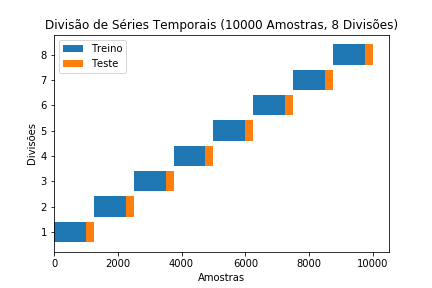
\includegraphics[scale=0.9]{monography/img/methods/blocking_cv.png}
    \label{figure:blocking}
    \caption[Representação do \textit{Out-of-Sample Testing} realizado]{Representação do \textit{Out-of-Sample Testing} realizado}
\end{figure}